\documentclass[11pt]{article}
\usepackage{tikz}

\begin{document}

\thispagestyle{empty}

\begin{center}

\begin{tikzpicture}
\foreach \n/\colorb/\colort in
  {-.5/40/50, 0/50/70, .5/70/40, 1/40/50, 1.5/50/70, 2.0/70/50, 2.5/50/40,%
   4/40/50, 4.5/50/70, 5/70/50, 5.5/50/40,%
   7/40/50, 7.5/50/40, 8/40/40,%
   8.5/40/50, 9/50/60,%
   10.5/50/50, 11/50/60, 11.5/60/70, 12/70/50, 12.5/50/40, 13/40/40}
    \shade[bottom color=black!\colorb,top color=black!\colort] (0,\n) rectangle +(5,5mm);
\draw[fill,color=black] (0,3) rectangle +(5,1);
\draw[fill,color=black] (0,6) rectangle +(5,1);
\draw[fill,color=black] (0,9.5) rectangle +(5,1);
\end{tikzpicture}
\end{center}

\newpage
\thispagestyle{empty}

\begin{center}

\begin{tikzpicture}
\draw[fill,color=gray]  (0,0) rectangle +(5,5);
\draw[fill,color=black] (0,5) rectangle +(5,5);
\end{tikzpicture}
\end{center}

\newpage
\thispagestyle{empty}

\begin{center}
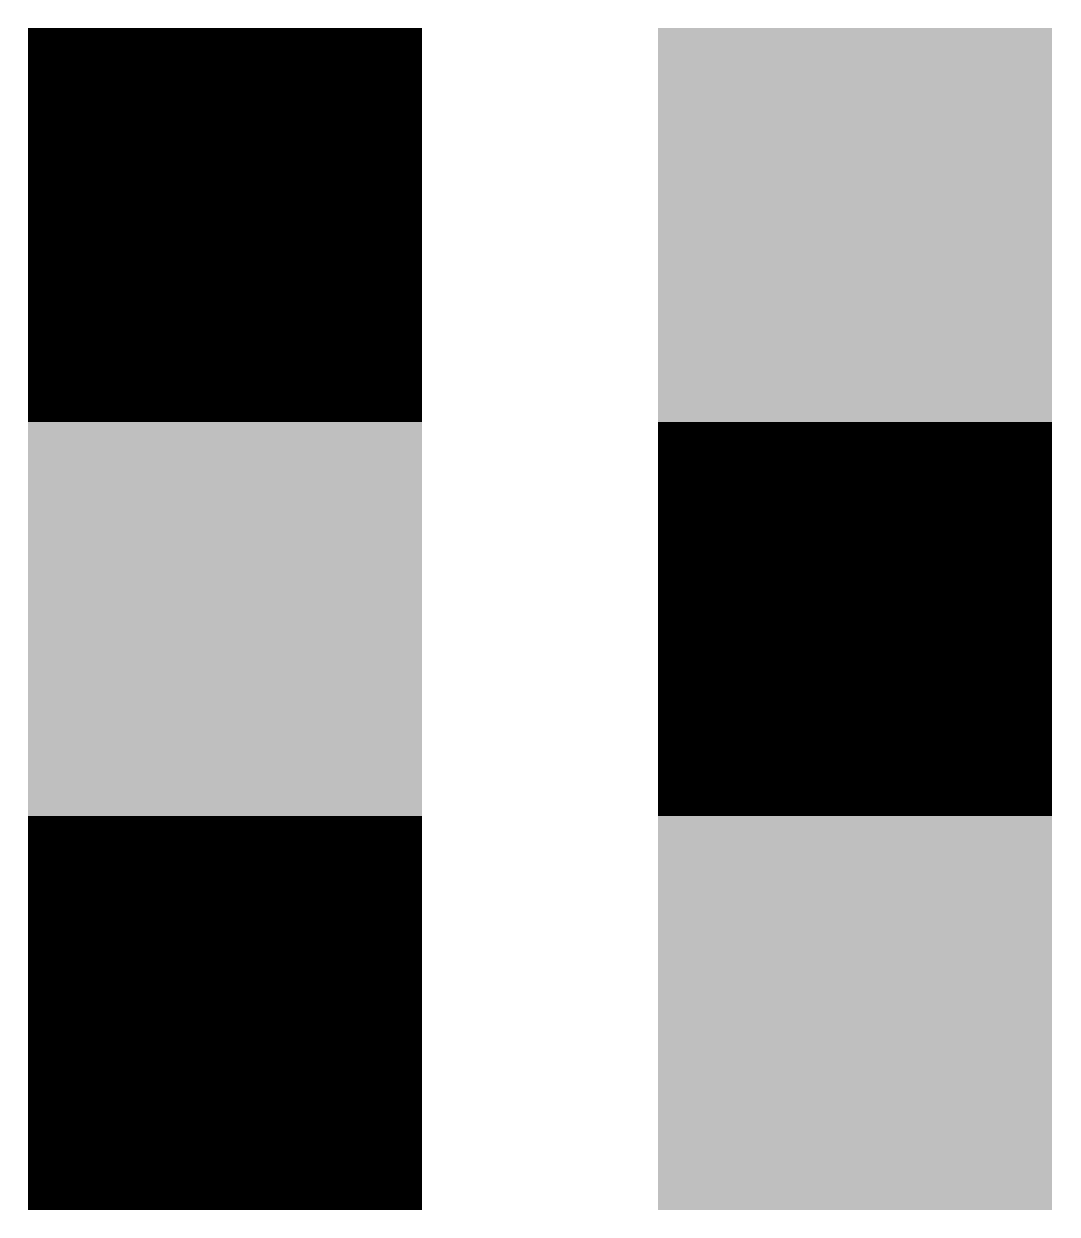
\begin{tikzpicture}
\draw[fill,color=black] (0,0) rectangle +(5,5);
\draw[fill,color=gray!50]  (0,5) rectangle +(5,5);
\draw[fill,color=black] (0,10) rectangle +(5,5);
\begin{scope}[xshift=8cm]
\draw[fill,color=gray!50] (0,0) rectangle +(5,5);
\draw[fill,color=black]  (0,5) rectangle +(5,5);
\draw[fill,color=gray!50] (0,10) rectangle +(5,5);
\end{scope}
\end{tikzpicture}
\end{center}

\newpage
\thispagestyle{empty}

\begin{center}

\begin{tikzpicture}
\draw[fill,color=gray!50]  (0,0) rectangle +(10,16);
\draw[fill,color=black] (0,4) rectangle +(6,8);
\end{tikzpicture}
\end{center}

\newpage
\thispagestyle{empty}

\begin{center}

\begin{tikzpicture}
\draw[fill,color=gray!50] (0,0) rectangle +(5,15);
\draw[fill,color=black]  (0,4) rectangle +(5,4);
\draw[fill,color=black]  (0,10.5) rectangle +(5,1.5);
\end{tikzpicture}
\end{center}

\end{document}
